\qquad O Merge Sort (ordenação por intercalação) é um algoritmo de
ordenação por comparação baseado no paradigma de \textit{dividir para
conquistar}: em vez de ordenar o vetor inteiro de uma só vez, ele o
divide em partes menores, ordena cada parte separadamente e, por fim,
combina os resultados. A ideia central é que \textit{intercalar}
(\textit{merge}) dois vetores que já estão ordenados é uma operação
simples e eficiente, pois basta comparar os elementos que estão no
início de cada um e ir retirando sempre o menor deles. Segundo Knuth
(1998), o método foi proposto por John von Neumann em 1945.

\qquad O algoritmo é executado, de forma recursiva, em três etapas:

\begin{enumerate}
    \item \textbf{Dividir:} o vetor é dividido ao meio, em duas metades
    de tamanhos (aproximadamente) iguais;
    \item \textbf{Conquistar:} cada metade é ordenada recursivamente,
    aplicando o próprio Merge Sort. A recursão termina quando o trecho
    possui um único elemento (ou nenhum), que já está ordenado por
    definição;
    \item \textbf{Combinar:} as duas metades, agora ordenadas, são
    intercaladas em um vetor auxiliar: compara-se o primeiro elemento
    ainda não utilizado de cada metade, copia-se o menor deles para o
    vetor auxiliar e avança-se naquela metade; quando uma das metades
    se esgota, copia-se o restante da outra; por fim, o trecho
    intercalado é copiado de volta para o vetor original.
\end{enumerate}

\qquad A seguir apresenta-se a implementação utilizada neste trabalho, em
C++, composta por três funções: \texttt{Intercalar}, que realiza a etapa
de combinação; \texttt{MergeSortRecursivo}, que realiza a divisão e as
chamadas recursivas; e \texttt{MergeSort}, ponto de entrada com a mesma
assinatura dos demais algoritmos do trabalho (vetor e tamanho), que
aloca o vetor auxiliar uma única vez:

\begin{verbatim}
void Intercalar(int *vetor, int *aux,
                int inicio, int meio, int fim) {
    int i = inicio, j = meio + 1, k = inicio;
    while (i <= meio && j <= fim) {
        if (vetor[i] <= vetor[j])
            aux[k++] = vetor[i++];
        else
            aux[k++] = vetor[j++];
    }
    while (i <= meio) aux[k++] = vetor[i++];
    while (j <= fim)  aux[k++] = vetor[j++];
    for (k = inicio; k <= fim; k++)
        vetor[k] = aux[k];
}

void MergeSortRecursivo(int *vetor, int *aux,
                        int inicio, int fim) {
    if (inicio >= fim) return;
    int meio = inicio + (fim - inicio) / 2;
    MergeSortRecursivo(vetor, aux, inicio, meio);
    MergeSortRecursivo(vetor, aux, meio + 1, fim);
    Intercalar(vetor, aux, inicio, meio, fim);
}

void MergeSort(int *vetor, int tamanho) {
    if (tamanho < 2) return;
    int *aux = new int[tamanho];
    MergeSortRecursivo(vetor, aux, 0, tamanho - 1);
    delete[] aux;
}
\end{verbatim}

\qquad Algumas características importantes do Merge Sort, que o distinguem
dos demais algoritmos deste trabalho:

\begin{itemize}
    \item \textbf{Desempenho previsível:} como a divisão e a intercalação
    são sempre executadas por completo, o custo é da ordem de
    $n \log n$ qualquer que seja a ordem inicial dos dados, ao contrário do
    Insertion e do Bubble Sort, que dependem do grau de ordenação da
    entrada;
    \item \textbf{Estabilidade:} o uso de \texttt{<=} na comparação faz com
    que, em caso de empate, o elemento da metade esquerda seja copiado
    primeiro, preservando a ordem relativa de elementos iguais;
    \item \textbf{Memória adicional:} é necessário um vetor auxiliar do
    mesmo tamanho do vetor original (cerca de 4 MB para 1.000.000 de
    inteiros), enquanto os outros quatro algoritmos ordenam no próprio
    vetor;
    \item \textbf{Profundidade da recursão:} como o vetor é dividido ao
    meio a cada chamada, a profundidade é de cerca de $\log_2 n$ níveis (20
    níveis para 1.000.000 de elementos), o que não representa risco de
    estouro de pilha.
\end{itemize}

\qquad Essas características são exploradas em detalhes na análise de
complexidade e nos resultados experimentais apresentados nas próximas
seções deste capítulo.

\subsection{Teste de Mesa Manual}

\qquad O teste de mesa manual do Merge Sort, apresentado na figura abaixo,
foi realizado à mão com um exemplo de entrada diferente dos exemplos
trabalhados em sala de aula, conforme exigido pelo enunciado do
trabalho, e mostra o estado do vetor a cada divisão e a cada
intercalação realizada.

\begin{figure}[htbp]
    \centering
    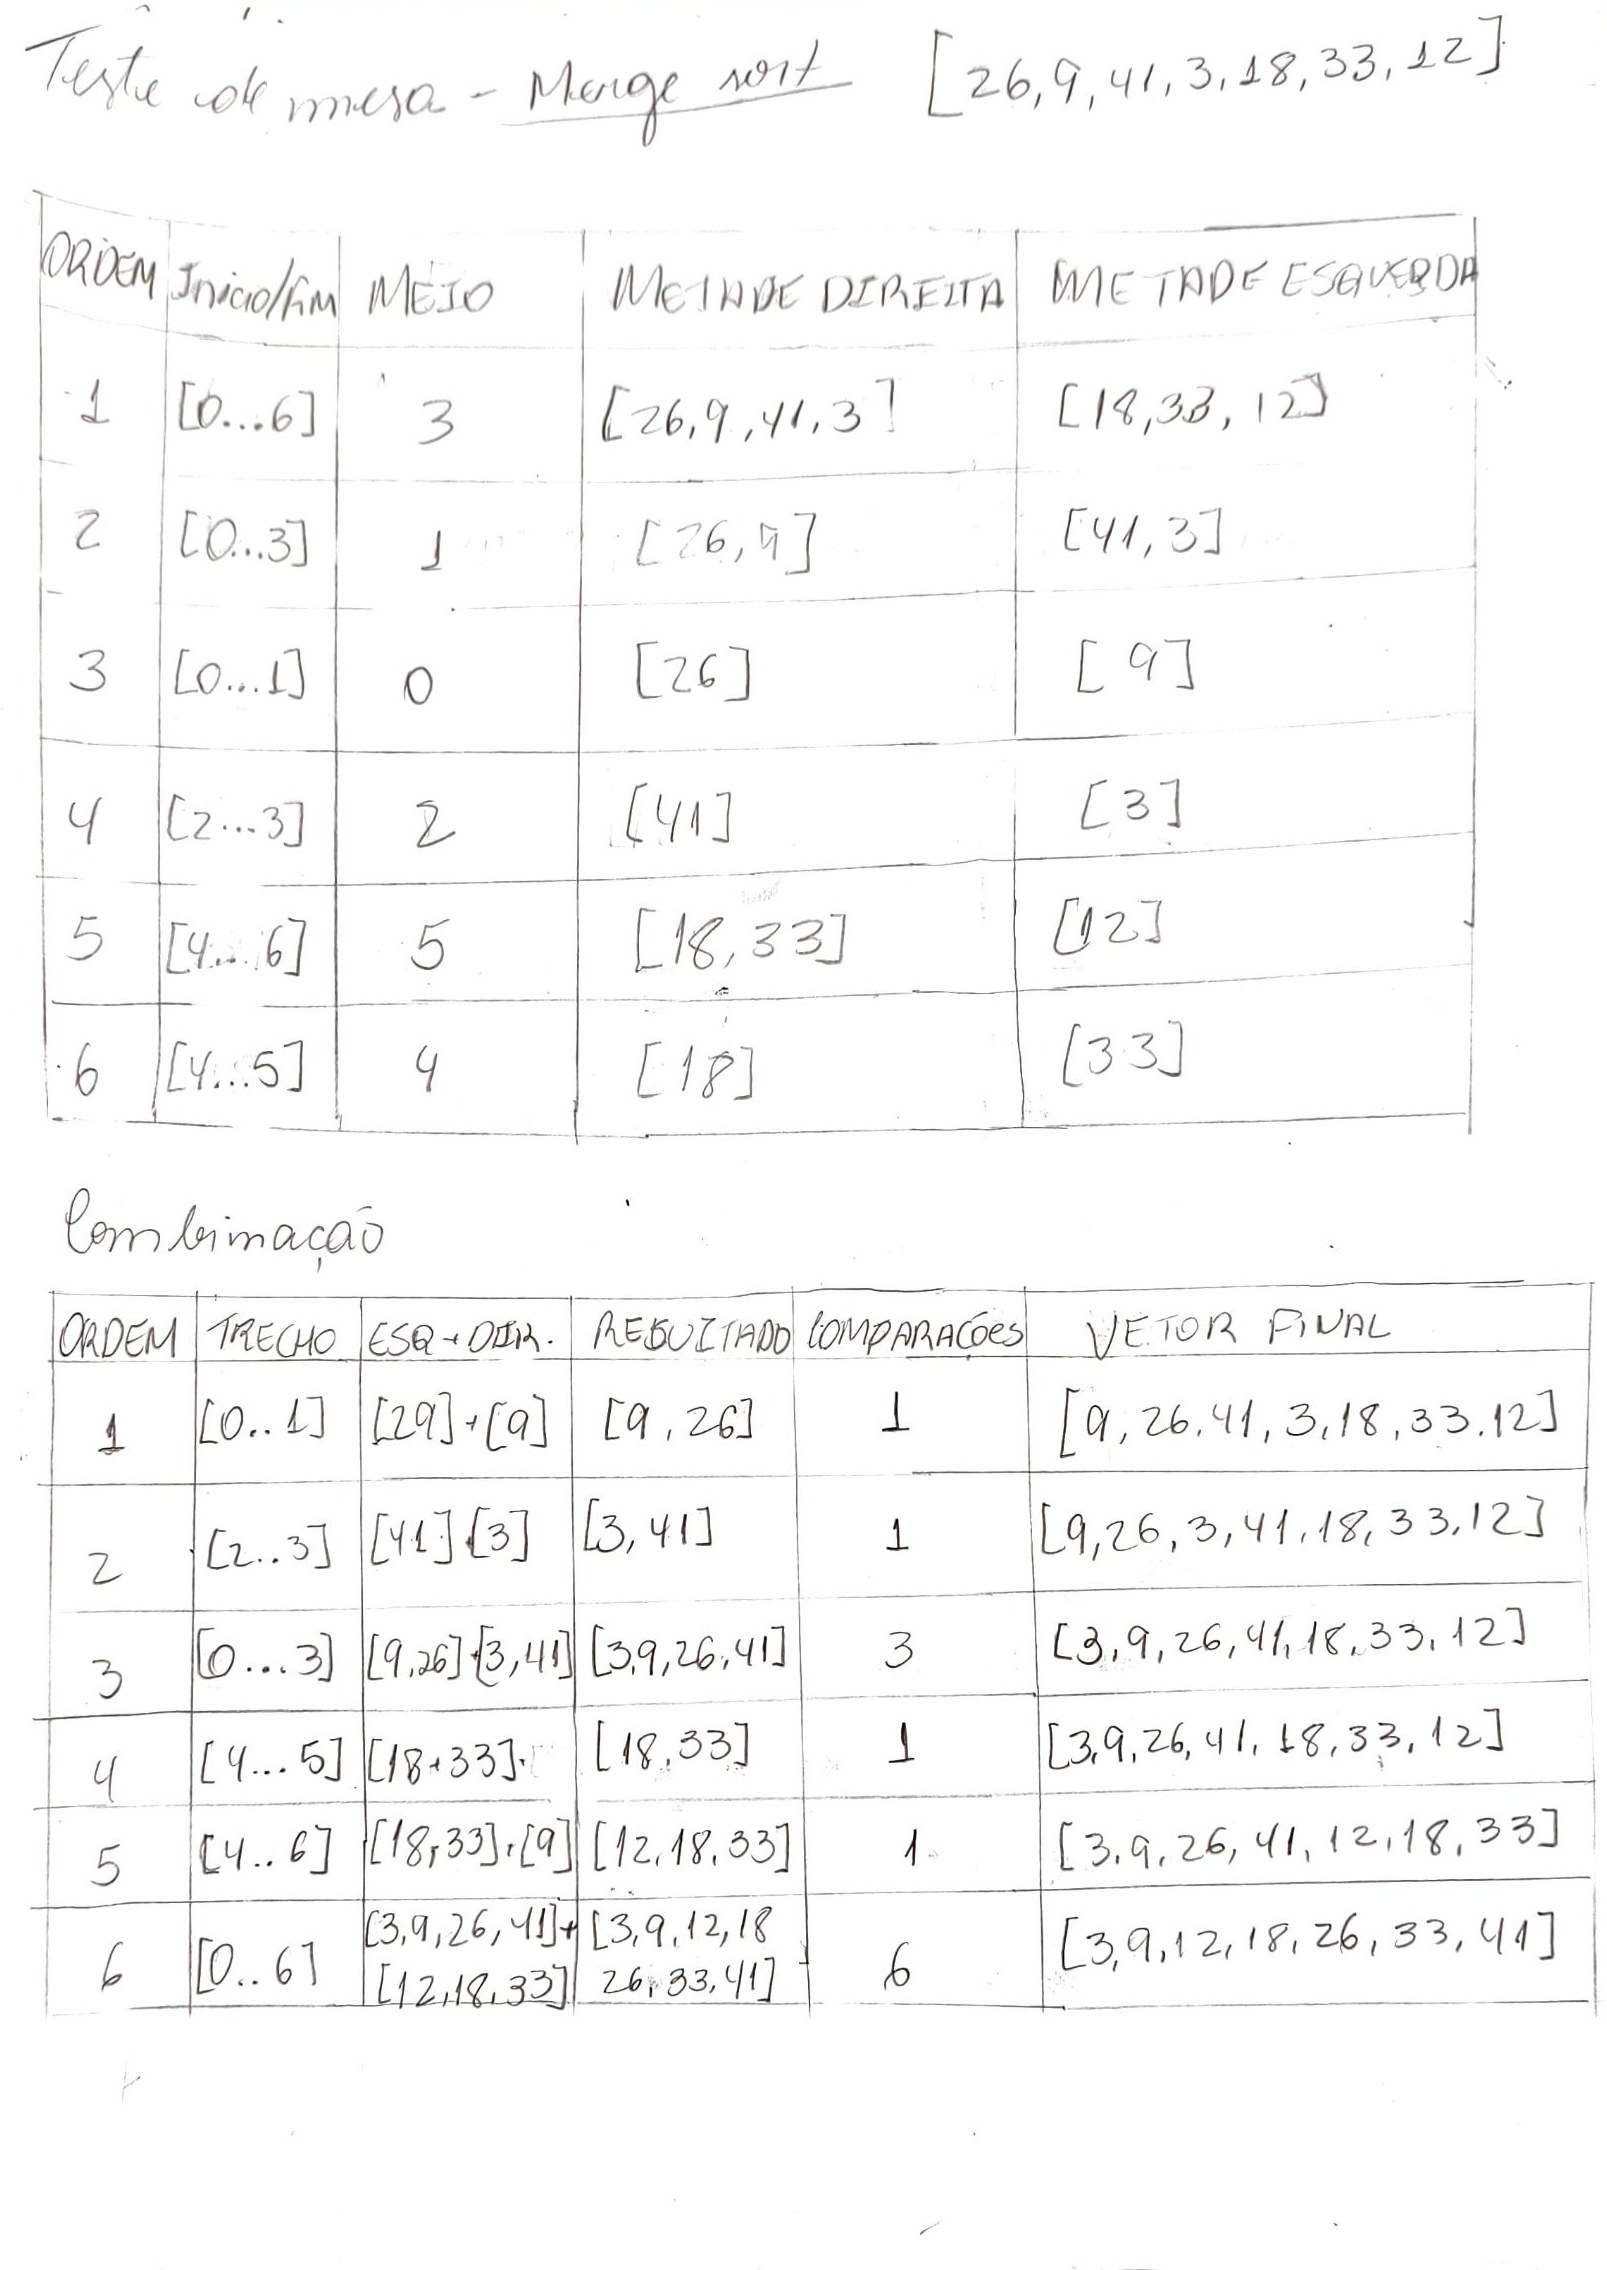
\includegraphics[width=14cm]{Imagens/Merge Sort/teste_de_mesa.png}
    \caption{Teste de mesa manual do algoritmo Merge Sort}
    \label{fig:teste_mesa_merge}
\end{figure}
